%%%%%%%%%%%%%%%%%%%%%%%%%%%%%%%%%%%%%%%%%%%%%%%%%%%%%%%%%%%%%%%%%%%%%%%%%%%%%
%% 03_arch_bus_concept.tex
%% Section: Bus Concept
%% Chapter: Architecture Concepts
%%
%% Describes the dual-bus architecture of the RWU-RV64I chip:
%%   - Wishbone B4 Classic for CPU-to-peripheral access
%%   - AMBA AXI4 (read-only subset) for cache-to-memory-arbiter path
%%
%% Integration in 00_rwurv64i_all.tex:
%%   \section{Bus Concept}
%%   \input{\TEXTarch 03_arch_bus_concept}
%%
%% Requires packages: tabularx, booktabs, tikz, float, xcolor, hyperref
%%
%% v0.1  2026-02-19  Claude-AI  Initial version (Wishbone only)
%% v0.2  2026-05-12  Claude-AI  Add AXI4 cache bus; dual-bus architecture
%%%%%%%%%%%%%%%%%%%%%%%%%%%%%%%%%%%%%%%%%%%%%%%%%%%%%%%%%%%%%%%%%%%%%%%%%%%%%

%%%%%%%%%%%%%%%%%%%%%%%%%%%%%%%%%%%%%%%%%%%%%%%%%%%%%%%%%%%%%%%%%%%%%%%%%%%%%
\subsection{Overview}
%%%%%%%%%%%%%%%%%%%%%%%%%%%%%%%%%%%%%%%%%%%%%%%%%%%%%%%%%%%%%%%%%%%%%%%%%%%%%

The RWU-RV64I chip uses a \textbf{dual-bus architecture} with two
independent on-chip buses serving different purposes:

\begin{itemize}
  \item \textbf{Wishbone B4 Classic} -- the peripheral bus.
    All configuration registers, GPIO, UART, and QSPI control registers
    are connected to the CPU via this bus.
    It was chosen for its simplicity, open-source IP availability, and
    compatibility with the existing peripheral IP blocks.

  \item \textbf{AMBA AXI4} (read-only subset) -- the cache memory bus.
    The I-Cache and D-Cache controllers use this bus to fetch 32-byte
    cache lines from NOR Flash via the Memory Arbiter and the QSPI
    controller data port.
    AXI4 was chosen for its burst capability: a 4-beat INCR burst fills
    one cache line in a single transaction instead of eight independent
    Wishbone single-cycle transfers.
\end{itemize}

The two buses are completely independent.
There is no bridge between them.
The Wishbone bus carries only single-word register accesses;
the AXI4 bus carries only 32-byte cache-line bursts.
Table~\ref{tab:asDualBus} summarises the key parameters of each bus.

\begin{table}[H]
\caption{On-Chip Bus Summary}
\label{tab:asDualBus}
\centering
\begin{tabularx}{\textwidth}{|l |X |X |X|}
  \hline
  Property          & Wishbone B4 Classic         & AXI4 (cache subset)      & Comment \\
  \hline
  \hline
  Purpose           & Peripheral access           & Cache line fill          & \\
  \hline
  Standard          & Wishbone B4 Classic         & AMBA AXI4                & \\
  \hline
  Data width        & 64\,bit                     & 64\,bit                  & \\
  \hline
  Address width     & 64\,bit                     & 32\,bit                  & Physical address only \\
  \hline
  Transfer type     & Single-word                 & 4-beat INCR burst        & ARLEN=3, ARSIZE=3 \\
  \hline
  Burst support     & No                          & Yes (read only)          & Write channels eliminated \\
  \hline
  Masters           & CPU core                    & I-Cache, D-Cache         & \\
  \hline
  Slaves            & GPIO, UART, QSPI cfg regs   & QSPI controller (data)   & \\
  \hline
  Arbitration       & Single master (no arbiter)  & Fixed priority (D $>$ I) & Memory Arbiter \\
  \hline
  Error signalling  & None (ERR\_O not driven)    & RRESP$\neq$OKAY          & Maps to RISC-V exceptions \\
  \hline
\end{tabularx}
\end{table}

%%%%%%%%%%%%%%%%%%%%%%%%%%%%%%%%%%%%%%%%%%%%%%%%%%%%%%%%%%%%%%%%%%%%%%%%%%%%%
\subsection{Bus Topology}
\label{subsec:asBusTopology}
%%%%%%%%%%%%%%%%%%%%%%%%%%%%%%%%%%%%%%%%%%%%%%%%%%%%%%%%%%%%%%%%%%%%%%%%%%%%%

Figure~\ref{fig:asBusTopology} shows the complete on-chip bus topology.
The two buses are rendered in different colours: Wishbone in blue,
AXI4 in red.
The QSPI controller is the only block that participates in both buses
(configuration registers on Wishbone, data port on AXI4).

\begin{figure}[H]
\centering
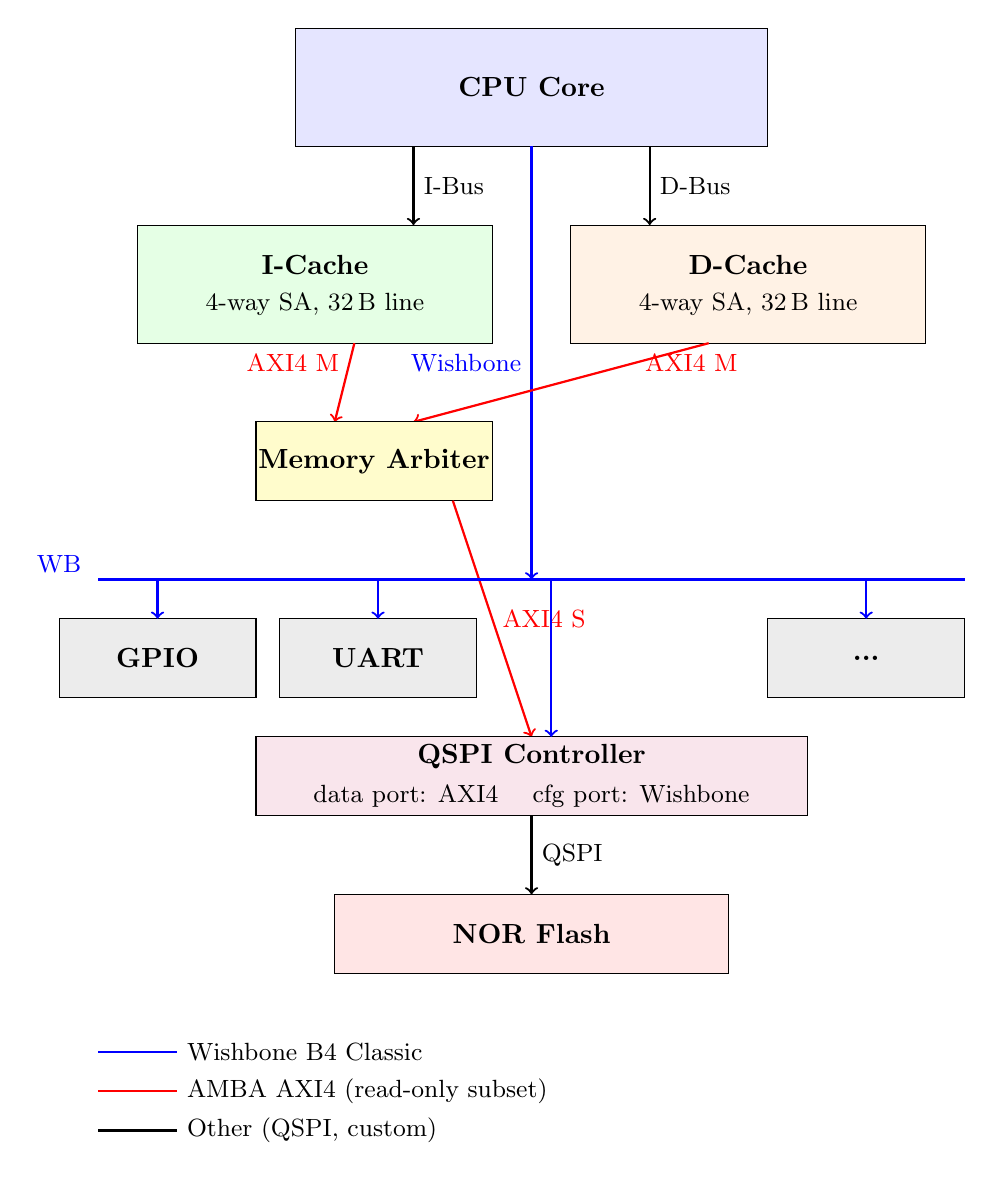
\begin{tikzpicture}[x=1cm, y=1cm]

  % ---- CPU Core ----
  \filldraw[fill=blue!10, draw=black] (3.0,13.0) rectangle (9.0,14.5);
  \node[align=center] at (6.0,13.75) {\textbf{CPU Core}};

  % I-Bus and D-Bus (custom, to caches)
  \draw[thick,->] (4.5,13.0) -- (4.5,12.0) node[midway,right,font=\small]{I-Bus};
  \draw[thick,->] (7.5,13.0) -- (7.5,12.0) node[midway,right,font=\small]{D-Bus};

  % Wishbone master port (CPU downward to WB bus)
  \draw[thick,blue,->] (6.0,13.0) -- (6.0,7.5)
    node[midway,left,font=\small,blue]{Wishbone};

  % ---- I-Cache ----
  \filldraw[fill=green!10, draw=black] (1.0,10.5) rectangle (5.5,12.0);
  \node[align=center] at (3.25,11.5) {\textbf{I-Cache}};
  \node[align=center,font=\small] at (3.25,11.0) {4-way SA, 32\,B line};

  % ---- D-Cache ----
  \filldraw[fill=orange!10, draw=black] (6.5,10.5) rectangle (11.0,12.0);
  \node[align=center] at (8.75,11.5) {\textbf{D-Cache}};
  \node[align=center,font=\small] at (8.75,11.0) {4-way SA, 32\,B line};

  % AXI4 from I-Cache to arbiter
  \draw[thick,red,->] (3.75,10.5) -- (3.5,9.5)
    node[near start,left,font=\small,red]{AXI4 M};

  % AXI4 from D-Cache to arbiter
  \draw[thick,red,->] (8.25,10.5)  -- (4.5,9.5)
    node[near start,right,font=\small,red]{AXI4 M};

  % ---- Memory Arbiter ----
  \filldraw[fill=yellow!20, draw=black] (2.5,8.5) rectangle (5.5,9.5);
  \node[align=center] at (4.0,9.0) {\textbf{Memory Arbiter}};

  % AXI4 from arbiter to QSPI
  \draw[thick,red,->] (5.0,8.5) -- (6.0,5.5)
    node[midway,right,font=\small,red]{AXI4 S};

  % ---- QSPI Controller ----
  \filldraw[fill=purple!10, draw=black] (2.5,4.5) rectangle (9.5,5.5);
  \node[align=center] at (6.0,5.25) {\textbf{QSPI Controller}};
  \node[align=center,font=\small] at (6.0,4.75) {data port: AXI4 \quad cfg port: Wishbone};

  % Wishbone to QSPI cfg port
  \draw[thick,blue,->] (6.25,7.5) -- (6.25,5.5);

  % QSPI bus to NOR Flash
  \draw[thick,->] (6.0,4.5) -- (6.0,3.5) node[midway,right,font=\small]{QSPI};

  % ---- NOR Flash ----
  \filldraw[fill=red!10, draw=black] (3.5,2.5) rectangle (8.5,3.5);
  \node[align=center] at (6.0,3.0) {\textbf{NOR Flash}};

  % ---- Wishbone Bus ----
  \draw[thick,blue] (0.5,7.5) -- (11.5,7.5);
  \node[blue,font=\small] at (0.0,7.7) {WB};

  % ---- GPIO ----
  \filldraw[fill=gray!15, draw=black] (0.0,6.0) rectangle (2.5,7.0);
  \node[align=center] at (1.25,6.5) {\textbf{GPIO}};
  \draw[thick,blue,->] (1.25,7.5) -- (1.25,7.0);

  % ---- UART ----
  \filldraw[fill=gray!15, draw=black] (2.8,6.0) rectangle (5.3,7.0);
  \node[align=center] at (4.05,6.5) {\textbf{UART}};
  \draw[thick,blue,->] (4.05,7.5) -- (4.05,7.0);

  % ---- ... ----
  \filldraw[fill=gray!15, draw=black] (9.0,6.0) rectangle (11.5,7.0);
  \node[align=center] at (10.25,6.5) {\textbf{...}};
  \draw[thick,blue,->] (10.25,7.5) -- (10.25,7.0);

  % Legend
  \draw[thick,blue] (0.5,1.5) -- (1.5,1.5);
  \node[right,font=\small] at (1.5,1.5) {Wishbone B4 Classic};
  \draw[thick,red]  (0.5,1.0) -- (1.5,1.0);
  \node[right,font=\small] at (1.5,1.0) {AMBA AXI4 (read-only subset)};
  \draw[thick]      (0.5,0.5) -- (1.5,0.5);
  \node[right,font=\small] at (1.5,0.5) {Other (QSPI, custom)};

\end{tikzpicture}
\caption{On-Chip Bus Topology -- Dual-Bus Architecture}
\label{fig:asBusTopology}
\end{figure}

%%%%%%%%%%%%%%%%%%%%%%%%%%%%%%%%%%%%%%%%%%%%%%%%%%%%%%%%%%%%%%%%%%%%%%%%%%%%%
\subsection{Bus Selection Rationale}
\label{subsec:asBusRationale}
%%%%%%%%%%%%%%%%%%%%%%%%%%%%%%%%%%%%%%%%%%%%%%%%%%%%%%%%%%%%%%%%%%%%%%%%%%%%%

Table~\ref{tab:asBusRationale} documents the decision to use a dual-bus
architecture rather than a single unified bus for all on-chip traffic.

\begin{table}[H]
\caption{Bus Selection Rationale}
\label{tab:asBusRationale}
\centering
\begin{tabularx}{\textwidth}{|l |X |X|}
  \hline
  Criterion & Wishbone (peripherals) & AXI4 (cache) \\
  \hline
  \hline
  Transfer pattern &
    Single register read/write; one word per transaction &
    32-byte cache line fill; 4 beats per transaction \\
  \hline
  Burst support &
    Not needed; register accesses are always single-word &
    Essential; without bursts, 8 independent transactions per
    cache miss instead of 1 \\
  \hline
  Latency &
    Zero wait states (combinatorial ACK); adequate for
    register accesses &
    Many cycles per miss; decoupled AR and R channels
    allow the QSPI controller to accept the address and
    then stream data without stalling the bus \\
  \hline
  Complexity &
    Very simple; no state machines required in the BPI &
    Higher; separate address/data channels, handshaking,
    ID tracking -- justified by the burst benefit \\
  \hline
  IP compatibility &
    All existing peripheral IP blocks use Wishbone;
    no changes required &
    Cache controllers are new IP; designed for AXI4 from
    the start \\
  \hline
  Write support &
    Full read/write (register access) &
    Read-only (write channels eliminated by MEM-01
    resolution; Flash is read-only) \\
  \hline
  Decision &
    \textbf{Keep Wishbone for all peripherals.}
    Adding AXI4 to GPIO/UART etc.\ would add complexity
    with no benefit. &
    \textbf{Use AXI4 for cache--memory path.}
    The 8$\times$ reduction in bus transactions per cache
    miss justifies the added complexity. \\
  \hline
\end{tabularx}
\end{table}

\input{\TEXTarchc 03_arch_bus_wishbone}

%%%%%%%%%%%%%%%%%%%%%%%%%%%%%%%%%%%%%%%%%%%%%%%%%%%%%%%%%%%%%%%%%%%%%%%%%%%%%
\subsection{AMBA AXI4 -- Cache Memory Bus}
\label{subsec:asAxi4Bus}
%%%%%%%%%%%%%%%%%%%%%%%%%%%%%%%%%%%%%%%%%%%%%%%%%%%%%%%%%%%%%%%%%%%%%%%%%%%%%

\subsubsection{Overview}

The AXI4 bus connects the two cache controllers (I-Cache and D-Cache)
through the Memory Arbiter to the QSPI controller data port.
It carries exclusively 32-byte cache-line read bursts.
Write channels (AW, W, B) are not instantiated: the AXI4 write path was
eliminated when the scratchpad SRAM replaced write-back-to-Flash
(MEM-01 resolution).

\subsubsection{Participants}

\begin{table}[H]
\caption{AXI4 Bus Participants}
\label{tab:asAxi4Participants}
\centering
\begin{tabularx}{\textwidth}{|l |l |X|}
  \hline
  Block & Role & Notes \\
  \hline
  \hline
  I-Cache controller & AXI4 Master (ID=0x1) &
    Issues read burst on cache miss; read-only \\
  \hline
  D-Cache controller & AXI4 Master (ID=0x2) &
    Issues read burst on cache miss; read-only \\
  \hline
  Memory Arbiter     & AXI4 Slave + Master &
    Accepts two masters; forwards one at a time to QSPI;
    fixed priority D-Cache $>$ I-Cache \\
  \hline
  QSPI controller (data port) & AXI4 Slave &
    Translates AXI4 read burst to Quad Fast Read SPI command;
    slow slave (many cycles per burst) \\
  \hline
\end{tabularx}
\end{table}

\subsubsection{Bus Parameters}

The AXI4 bus uses a reduced parameter set:
all transfers are fixed-length 4-beat INCR read bursts.

\begin{table}[H]
\caption{AXI4 Cache Bus Parameters}
\label{tab:asAxi4BusParams}
\centering
\begin{tabularx}{\textwidth}{|l |l |X|}
  \hline
  Parameter & Value & Comment \\
  \hline
  \hline
  Protocol       & AXI4 (not AXI4-Lite)   & Burst support required \\
  \hline
  Data width     & 64\,bit                 & One RV64 doubleword per beat \\
  \hline
  Address width  & 32\,bit                 & Physical address (\texttt{PA\_WIDTH=32}) \\
  \hline
  ID width       & 4\,bit                  & I-Cache: \texttt{4'h1}; D-Cache: \texttt{4'h2} \\
  \hline
  Burst type     & INCR only               & Sequential address; no WRAP, no FIXED \\
  \hline
  Burst length   & ARLEN = 3               & 4 beats $\times$ 8\,B = 32\,B per cache line \\
  \hline
  Beat size      & ARSIZE = 3              & 8 bytes per beat \\
  \hline
  Channels used  & AR, R only              & AW, W, B channels not instantiated \\
  \hline
  Outstanding tx & 1 per master            & Each cache has at most 1 transaction in flight \\
  \hline
\end{tabularx}
\end{table}

The full AXI4 channel signal definitions, the SystemVerilog interface
\texttt{as\_axi4\_if}, and the AXI4 timing diagrams are documented in
the Memory Concept section (Section~``Memory Concept'',
subsection ``AXI4 Memory Bus'').

\subsubsection{QSPI Controller -- Dual Bus Participation}

The QSPI controller is the only block that participates in both buses:

\begin{itemize}
  \item \textbf{AXI4 slave port (data):}
    Receives 4-beat INCR read bursts from the Memory Arbiter.
    Translates each burst into a Quad Fast Read (\texttt{0x6B})
    command sequence on the SPI bus and returns 32 bytes in 4 AXI4
    R-channel beats.
    This port is part of the AXI4 cache memory bus.

  \item \textbf{Wishbone slave port (configuration):}
    Receives single-word register accesses from the CPU for
    QSPI mode configuration, status readback, and manual SPI command
    injection.
    This port is part of the Wishbone peripheral bus and uses the
    standard \texttt{as\_slave\_bpi} wrapper.
\end{itemize}

The two ports are independent and may be active simultaneously.
The QSPI controller arbitrates internally between the AXI4 data path
and the Wishbone configuration path, with the AXI4 burst taking
priority over a concurrent Wishbone access.

\input{\TEXTarchc 03_arch_bus_slavebpi}

%%%%%%%%%%%%%%%%%%%%%%%%%%%%%%%%%%%%%%%%%%%%%%%%%%%%%%%%%%%%%%%%%%%%%%%%%%%%%
\subsection{Bus Interconnect}
\label{subsec:asBusInterconnect}
%%%%%%%%%%%%%%%%%%%%%%%%%%%%%%%%%%%%%%%%%%%%%%%%%%%%%%%%%%%%%%%%%%%%%%%%%%%%%

\subsubsection{Two Independent Buses}

The Wishbone and AXI4 buses are completely separate.
There is no bridge, no shared wires, and no arbitration between them.
Traffic routing is determined at design time by which port of each block
is connected to which bus:

\begin{itemize}
  \item All CPU accesses to peripheral registers use the Wishbone bus.
  \item All cache-line fills use the AXI4 bus.
  \item The QSPI controller has one port on each bus; they operate
    independently.
\end{itemize}

\subsubsection{Wishbone Address Map}

Each Wishbone slave is mapped to a contiguous, non-overlapping region of
the address space.
Address decoding is performed by the bus interconnect logic, which
forwards \texttt{STB} and \texttt{CYC} only to the addressed slave.
Slaves whose address range is not selected must drive \texttt{ACK\_O}
low and \texttt{DAT\_O} to zero.
The actual address boundaries are defined in the chip-level memory map
(Chapter~``Memory Map and Registers'').

\subsubsection{Wishbone Topology}

The current Wishbone implementation uses a \textbf{shared bus} topology
with a single master (the CPU core).
A crossbar switch is not implemented because there is currently only one
Wishbone master and the zero-wait-state slave design means bus bandwidth
is limited only by the clock frequency.
If a DMA controller is added, its data buffers should be placed in the
Scratchpad SRAM (which is not a Wishbone slave), not on the Wishbone bus,
so the Wishbone topology does not need to change.

\subsubsection{AXI4 Topology}

The AXI4 bus uses a simple \textbf{Memory Arbiter} (two masters, one slave):
I-Cache and D-Cache are both AXI4 masters; the QSPI controller data port
is the single AXI4 slave.
The arbiter implements fixed priority (D-Cache $>$ I-Cache) and never
interrupts an in-progress burst.
Details are documented in the Memory Concept section.

\subsubsection{Peripheral Register Offset Alignment}

All peripheral registers are 64\,bit wide and aligned to 8-byte boundaries.
The address offset within a peripheral starts at \texttt{0x00} for the
ID register and increases in steps of \texttt{0x08}.
This is consistent with the Wishbone bus data width and the 64-bit
alignment of the RISC-V load and store instructions used to access the
peripheral registers.

\subsubsection{Read-Modify-Write}

The Wishbone protocol as implemented does not support atomic
read-modify-write operations.
Software must therefore use disable-interrupt / critical-section
patterns when accessing shared registers from multiple contexts.

%%%%%%%%%%%%%%%%%%%%%%%%%%%%%%%%%%%%%%%%%%%%%%%%%%%%%%%%%%%%%%%%%%%%%%%%%%%%%
\subsection{Comparison: Wishbone vs.\ AXI4}
%%%%%%%%%%%%%%%%%%%%%%%%%%%%%%%%%%%%%%%%%%%%%%%%%%%%%%%%%%%%%%%%%%%%%%%%%%%%%

Table~\ref{tab:asBusCompare} summarises the key differences between the
two on-chip buses and the rationale for using each.

\begin{table}[H]
\caption{Wishbone B4 Classic vs.\ AXI4 -- Key Differences}
\label{tab:asBusCompare}
\centering
\begin{tabularx}{\textwidth}{|l |X |X|}
  \hline
  Property & Wishbone B4 Classic & AXI4 (cache subset) \\
  \hline
  \hline
  Transfer unit     & 1 word (64\,bit)        & 4 beats $\times$ 64\,bit = 32\,B \\
  \hline
  Channels          & Shared address/data     & Decoupled AR and R \\
  \hline
  Handshake         & STB + ACK               & VALID + READY per channel \\
  \hline
  Outstanding tx    & 0 (blocking)            & 1 per master \\
  \hline
  Burst             & Not supported           & INCR, 4 beats fixed \\
  \hline
  Write support     & Full                    & None (write channels removed) \\
  \hline
  Error signalling  & None                    & RRESP; maps to RISC-V exceptions \\
  \hline
  Latency model     & 0 wait states typical   & Variable; QSPI controller stalls until Flash data arrives \\
  \hline
  Complexity        & Minimal                 & Moderate (5 channels, ID tracking, burst counter) \\
  \hline
  Used for          & Peripheral registers    & Cache-line fills from NOR Flash \\
  \hline
\end{tabularx}
\end{table}

